\documentclass[CMPE]{KGCOEReport}

\usepackage{graphicx}
\usepackage{newtxtext, newtxmath}
\usepackage{parskip}
\usepackage{karnaugh-map}
\usepackage{float}
\usepackage{pdfpages}

\graphicspath{{./assets/}}

\newcommand{\classCode}{CMPE 250}
\newcommand{\name}{Aden Perry}
\newcommand{\LabSectionNum}{L1}
\newcommand{\LabInstructor}{Chongzhou Fang}

\newcommand{\TAs}{Eddie Satowski \\ Eric Reed \\ Khoi Pham}
\newcommand{\LectureSectionNum}{01}
\newcommand{\LectureInstructor}{Chongzhou Fang}
\newcommand{\exerciseNumber}{8}
\newcommand{\exerciseDescription}{Multiprecision Arithmetic}
\newcommand{\dateDone}{2026-03-19}
\newcommand{\dateSubmitted}{2025-03-28}

\begin{document}

\maketitle

\section*{Abstract}

The purpose of this exercise was to design a program written in Keil ARM-v6-M
Assembly using the Thumb 1 instruction set capable of performing addition
operations on numbers of arbitrary word length stored in memory. The ADCS
instruction was used to add successive word chunks of the number while
respecting the Carry flag. A basic TUI was implemented to get an n-word number
from a user; user input was case-insensitive, and leading zeroes were optional.
The program was tested with various inputs to ensure overflow, carry, and
inputs of different lengths worked as expeceted. The exercise was successful,
as all test inputs produced the correct outputs.

\section*{Procedure}


\section*{Results}


\section*{Conclusion}


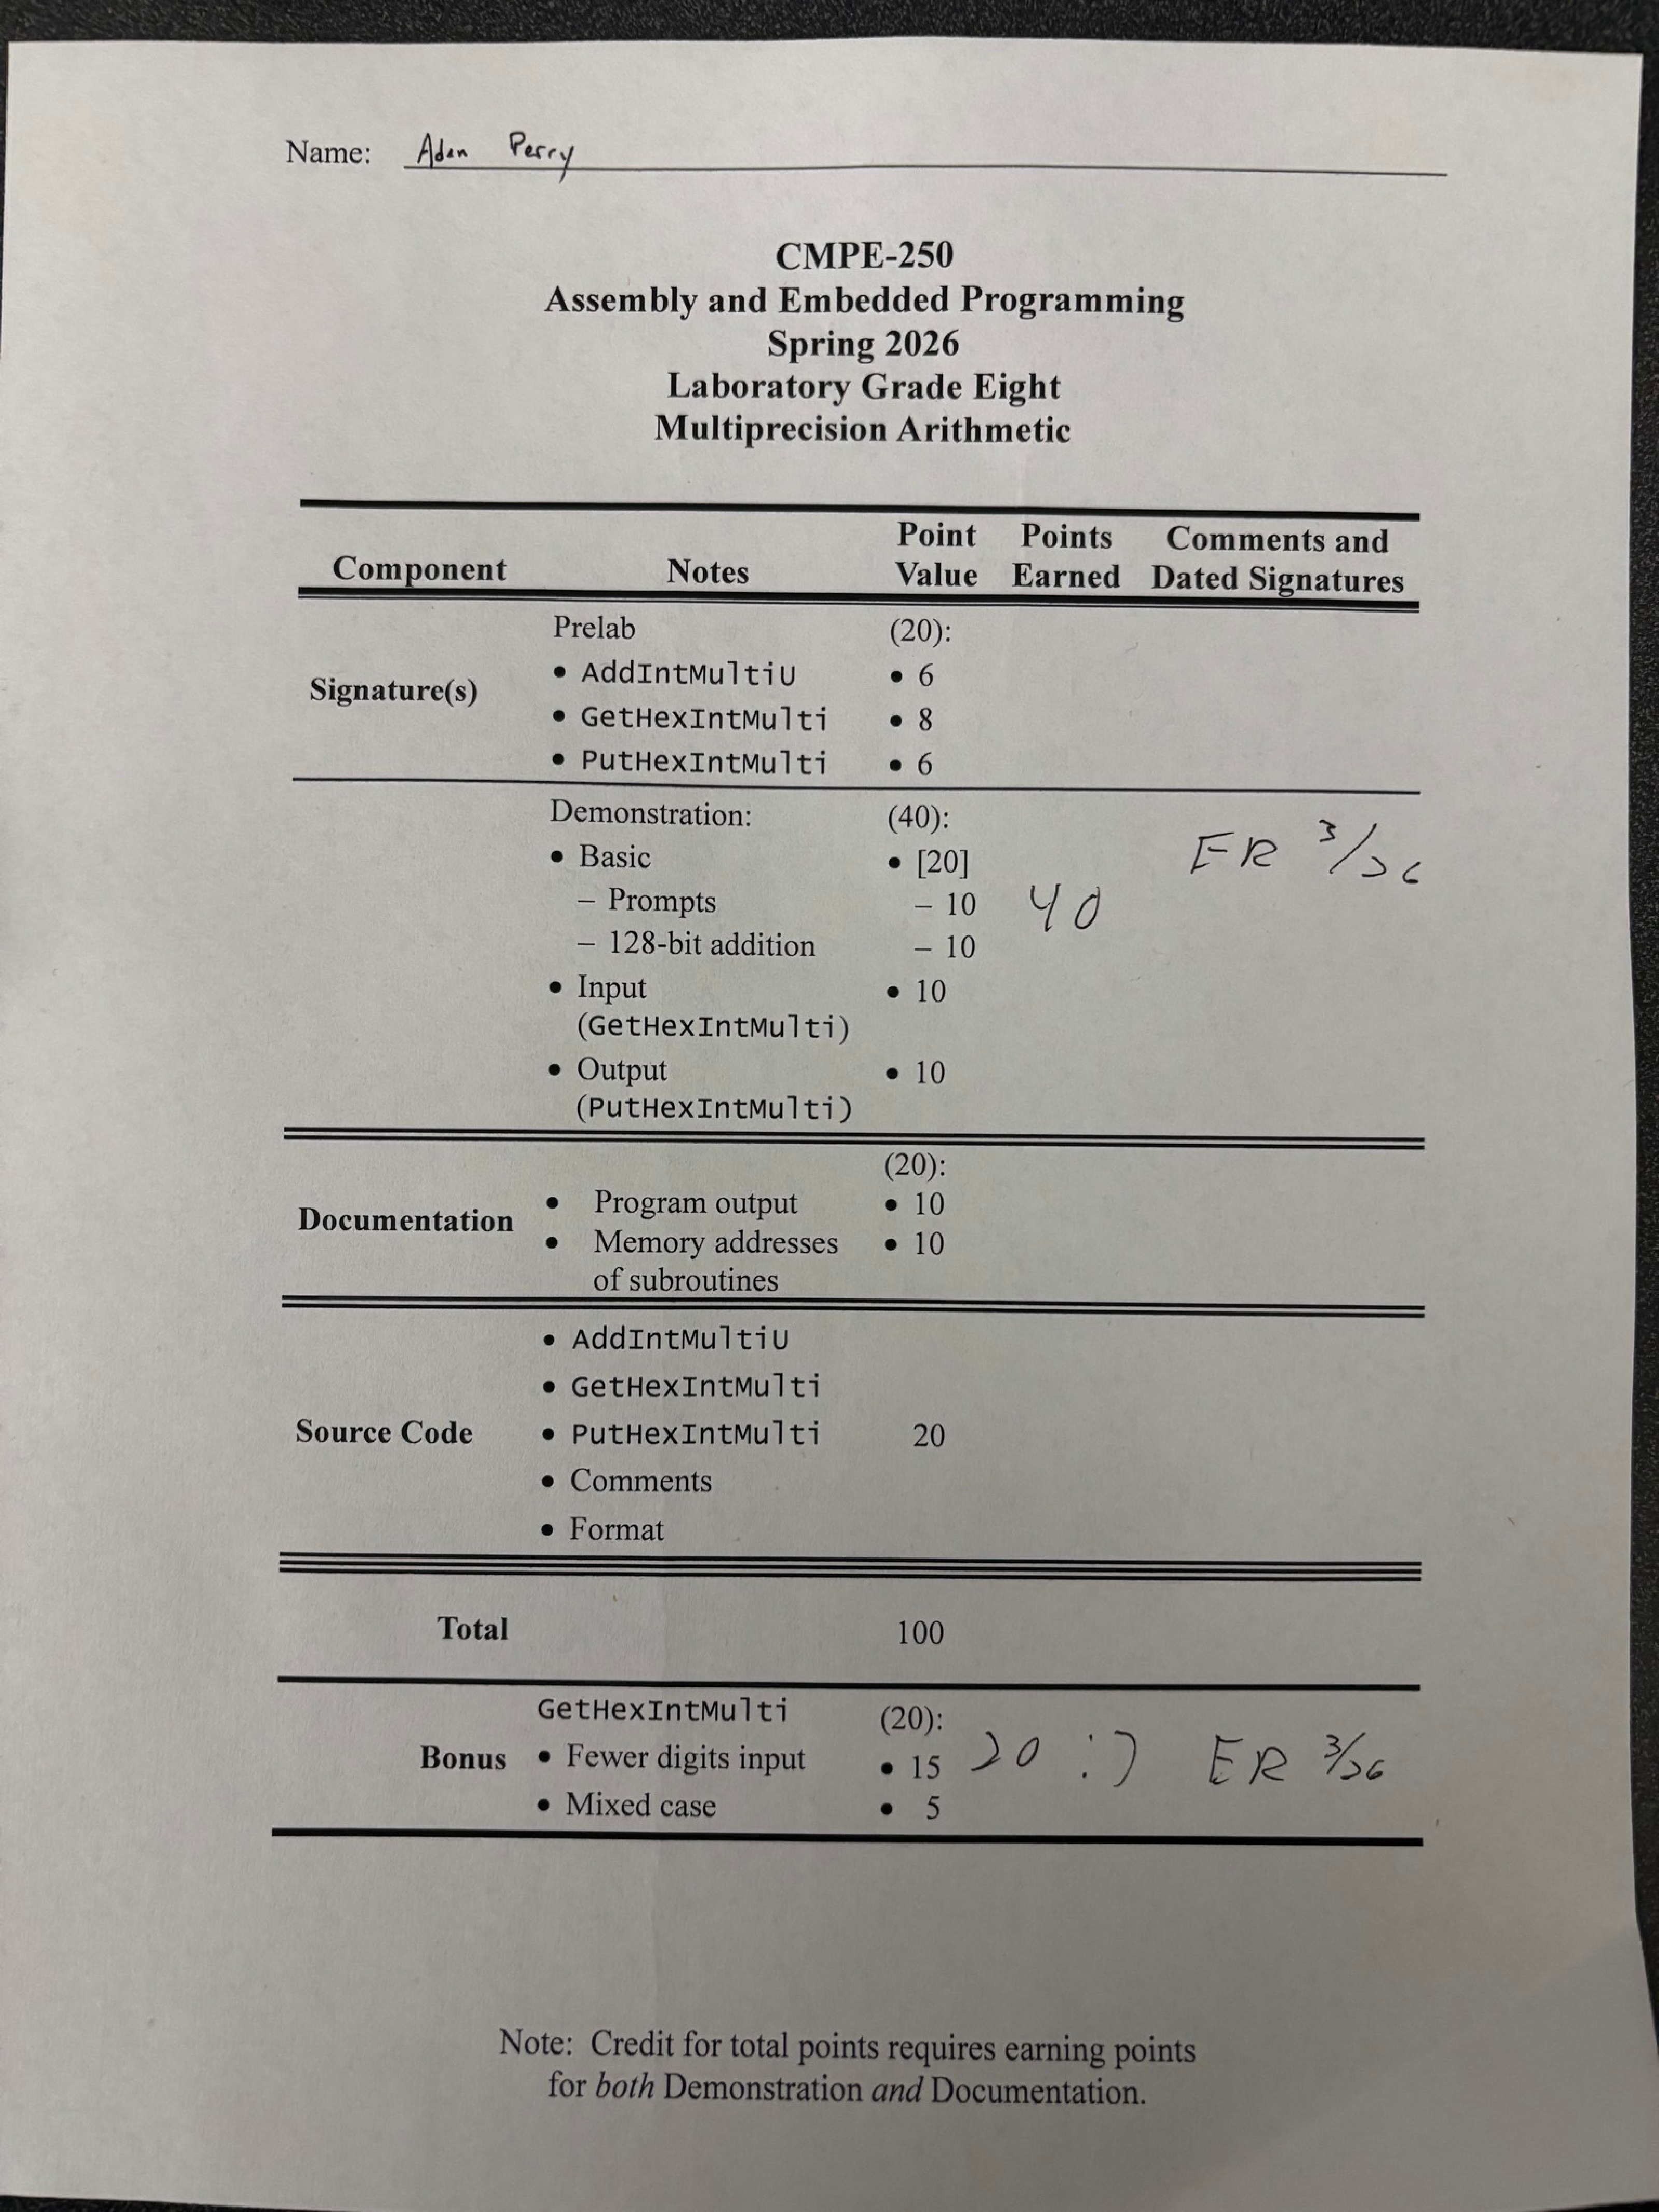
\includepdf[pages=-]{assets/prelab}

\end{document}
